%************************************************
\chapter{The data}\label{ch:mathtest} % $\mathbb{ZNR}$
%************************************************
Night-time lights data are released by NASA and the EOG project of the Colorado School of Mines. Data is published with different timeframes, i.e. nightly, monthly and yearly.
As I will illustrate in this chapter, the data need to be cleaned before being used, and the two sources use different data cleaning algorithms; NASA has a faster publishing rate. New data is released each night just over an hour after the satellite took the imagery. On the other hand, the EOG data, from the analysis I have carried out, implements a more effective data cleaning algorithm. Moreover, NASA files are published in tiles, small portions of space that must be processed before they can be used. Each tile must be geolocalised in space according to the order in which the tile is positioned.

\section{Dealing with satellite data}

Night-Time light data are distributed in georeferenced \textit{.tif} images, which are images that contain map projection information, namely the coordinate reference system. 
\textit{Raster} files are  $n \times k$  matrices that divide the observation surface into rectangular pixels.

\begin{figure}[h]
    \begin{center}
    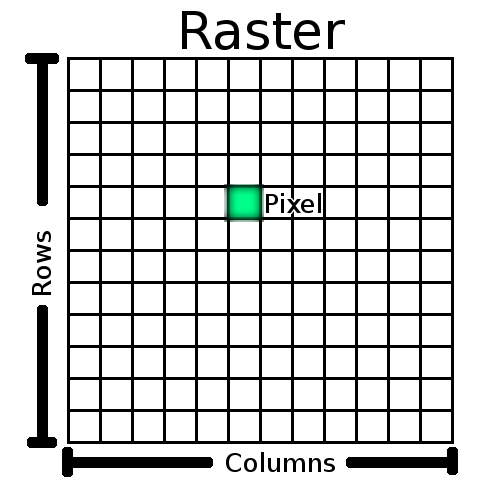
\includegraphics[width=7cm]{images/raster_dataset.png}
    \end{center}
    \caption{Raster representation - Source: Qgis Documentation.}
\end{figure}


With night-time lights, each cell of the raster matrix contains the reflectance measured in that specific portion of the globe.
Depending on the sensor's technology mounted on the satellite, the pixels will capture smaller portions of the globe, producing higher resolution images. 

Given the circular motion of the satellite orbit, the resolution is measured in \textit{arc/seconds}. Regarding the two main technologies in the night-time lights industry, the VIIRS sensor data has a resolution of 15 arc/seconds (circa 500 metres at the equator), while the previous DMSP sensor data is about 30 arc/seconds (circa 1000 metres at the equator). 
\begin{figure}[h]
    \begin{center}
    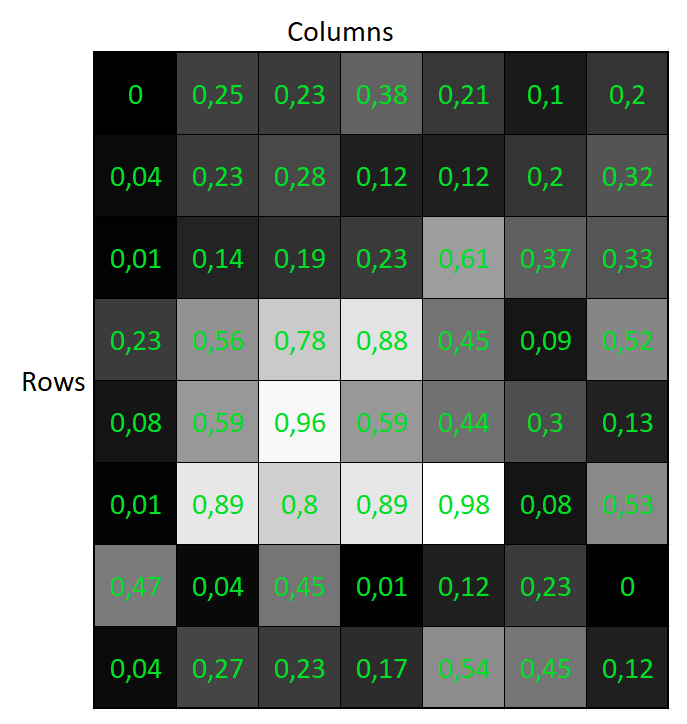
\includegraphics[width=7cm]{images/raster_night.png}
    \end{center}
    \caption{Night-time raster representation.}
\end{figure}
The geographic reference system divides the Earth into 360 equal segments called degrees. Each degree contains 60 minutes and, therefore, 3600 seconds.
An arc-second is the geographical distance measured on the surface of the Earth after one second's rotation, or 1/3600th of a degree.
At the equator, one arc/second of latitude corresponds in metres to one arc/second of longitude. However, the further one moves towards the poles, the equivalent of one arc/second in longitude decreases while latitude remains stable.
  
To perform \textit{zonal statistics}, i.e. statistics of delimited areas of the globe, it is necessary to delimit the raster files with another file that contains georeferenced information about geographical boundaries. For this purpose, most of the time, \textit{Shapefiles} or \textit{GeoJson} are used, which are called "polygon files". These files contain information about the boundaries of the geographical regions to be studied. As with raster files, polygon files can also have different resolutions. In this thesis, I will use the data with the highest possible resolution distributed by GADM.
\begin{figure}[h]
    \begin{center}
    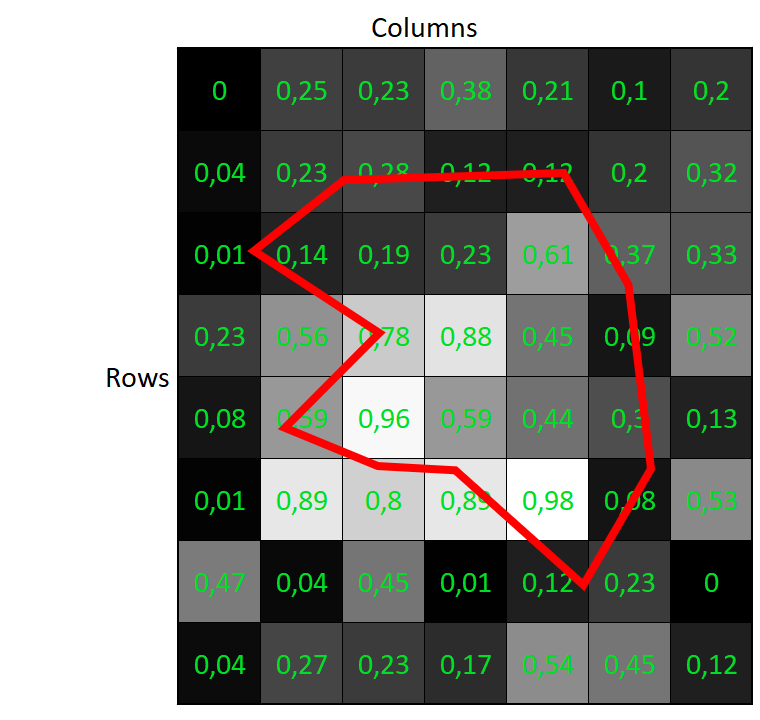
\includegraphics[width=7cm]{images/raster_night_cover.png}
    \end{center}
    \caption{Night-time lights extraction process representation.}
    \label{fig:extraction}
\end{figure}
GADM is a free open-access database of global administrative areas that publishes high-quality border data.
The geographical area to be studied is obtained from the intersection of the raster file and the polygon file such that a statistical function can be applied. For this thesis, I will make use of summation, but spatial variance can be used as well.
Given a $m\times n$ raster file, the summation is defined as:
\begin{equation}
    TotNTL=\sum_{i=1}^n\sum_{j=1}^m x_{ij}.
\end{equation}
An important consideration must be made regarding the data extraction process. It is legitimate to ask how to deal with pixel values only partially contained within the geographical boundaries of interest as in \autoref{fig:extraction}. In this thesis, I will use the R package {\it exactextractr}, which is the most refined package for data extraction. This package, unlike {\it raster} and {\it terra} alternatives, extracts values by weighting them for effective coverage. 
A final note on the analysed data is the weight they occupy on the disk. An annual panel analysis of 11 years results in a data volume of around 120 gigabytes multiplied by 12 (i.e. around 1.5 terabytes) if the analysis is carried out with monthly data. This results into long analysis processes and so high computing power is needed.

\section{Data problems}
Managing satellite data is complex. One of the difficulties is dealing with some capturing issues that, without correction, may give biased data. For this reason, research on the best algorithms for cleaning and producing data does not stop, and new types of algorithms are constantly updated. The three main problems we face are:
\begin{enumerate}
\item \textbf{Cloud Coverage:} As argued earlier, one of the many purposes of night-time lights was to study the presence of clouds. It is, therefore, not surprising that, if only interested in the dynamics of the emitted night-time illumination, the complete or partial overlay of clouds may result in missing or dirty data. 
The data published by both NASA and EOG also include detailed information on the areas where clouds were present at the time of the capture. It is up to the researcher to choose whether the amount of daily data without cloud cover is sufficient for her purposes. 
A possible solution is to use the information on the areas covered by clouds from other periods. To do this, the time window of analysis must be increased. Several algorithms have been developed to aggregate daily data into monthly or annual surveys. 
The operation is not complex and works as follows, given several daily surveys in one layer of raster information and another layer with the different cloud cover of the respective days, the algorithm takes only the values of the non-covered or partially covered areas and through a statistical function (mean or median most of the time) reconstructs a complete image.
Although very rare, a particular area may be covered for a whole month by clouds that prevent a correct representation of the actual light emitted. For this reason, it is necessary to consider the percentage of cloud-free observations of that month. Otherwise, data would be biased and annual aggregates may have to be used.
\item \textbf{Natural lights:} when measuring night-time lights, the presence of natural lights is a problem. Natural lights include sunlight, moonlight, reflections, burning biomass and other ephemeral events.
Dealing with these problems is much more complex than with cloud coverage. Different strategies have been adopted.
The most common of the strategies is cleaning through data aggregation, as seen above. This is because some of these natural lights have a seasonal nature. For instance, some areas of Northern Europe in the summer months suffer from overexposure to light at night, and the resulting images have entire areas burnt out. This kind of problem can be solved satisfactorily by aggregating an entire year's daily images.
On the other hand, other natural light sources have no seasonal character, namely, among the others, burning biomass and reflections. In this case, the remote sensing literature has treated these problems as outliers and proposed some solutions. For instance, the first version of EOG data used a histogram-based technique in which the tails were cut off. This data was further cleaned by eliminating background noise by identifying a minimum threshold in the neighbourhood of each pixel.
\item \textbf{Stray Lights:} In optics, stray lights are defined as instrumental noise in optical systems due to unwanted light, namely reflections or lens imperfections. Again, various algorithms have been created to deal with this issue. EOG publishes two types of data, "vcm" is the raw non-stray light corrected data, while "vcmsl" is the cleaned data.
\end{enumerate}
The data I will use in this thesis are those of the EOG project. In the last years, they adopted three versions of the cleaning algorithm, V1.0, V2.0, and V2.1, which have gradually become more and more sophisticated in handling the issues mentioned above.
Version 2.0 of the algorithm updates the threshold detection used to eliminate the light background in a sophisticated manner. Without intending to be exhaustive, the new algorithm calculates the median of the maximum values of the multiyear time series, weighted for cloud-free observations. A scattergram of the observations is then created by plotting the percentage of cloud free versus the data range, and a gamma curve was fit to lie above the scattergram noise levels. Gamma curves are usually adopted in optics applications. In this case, the gamma curve sets a threshold for each globe observation for each cloud-coverage level. 
\begin{figure}[h!]
    \centering
    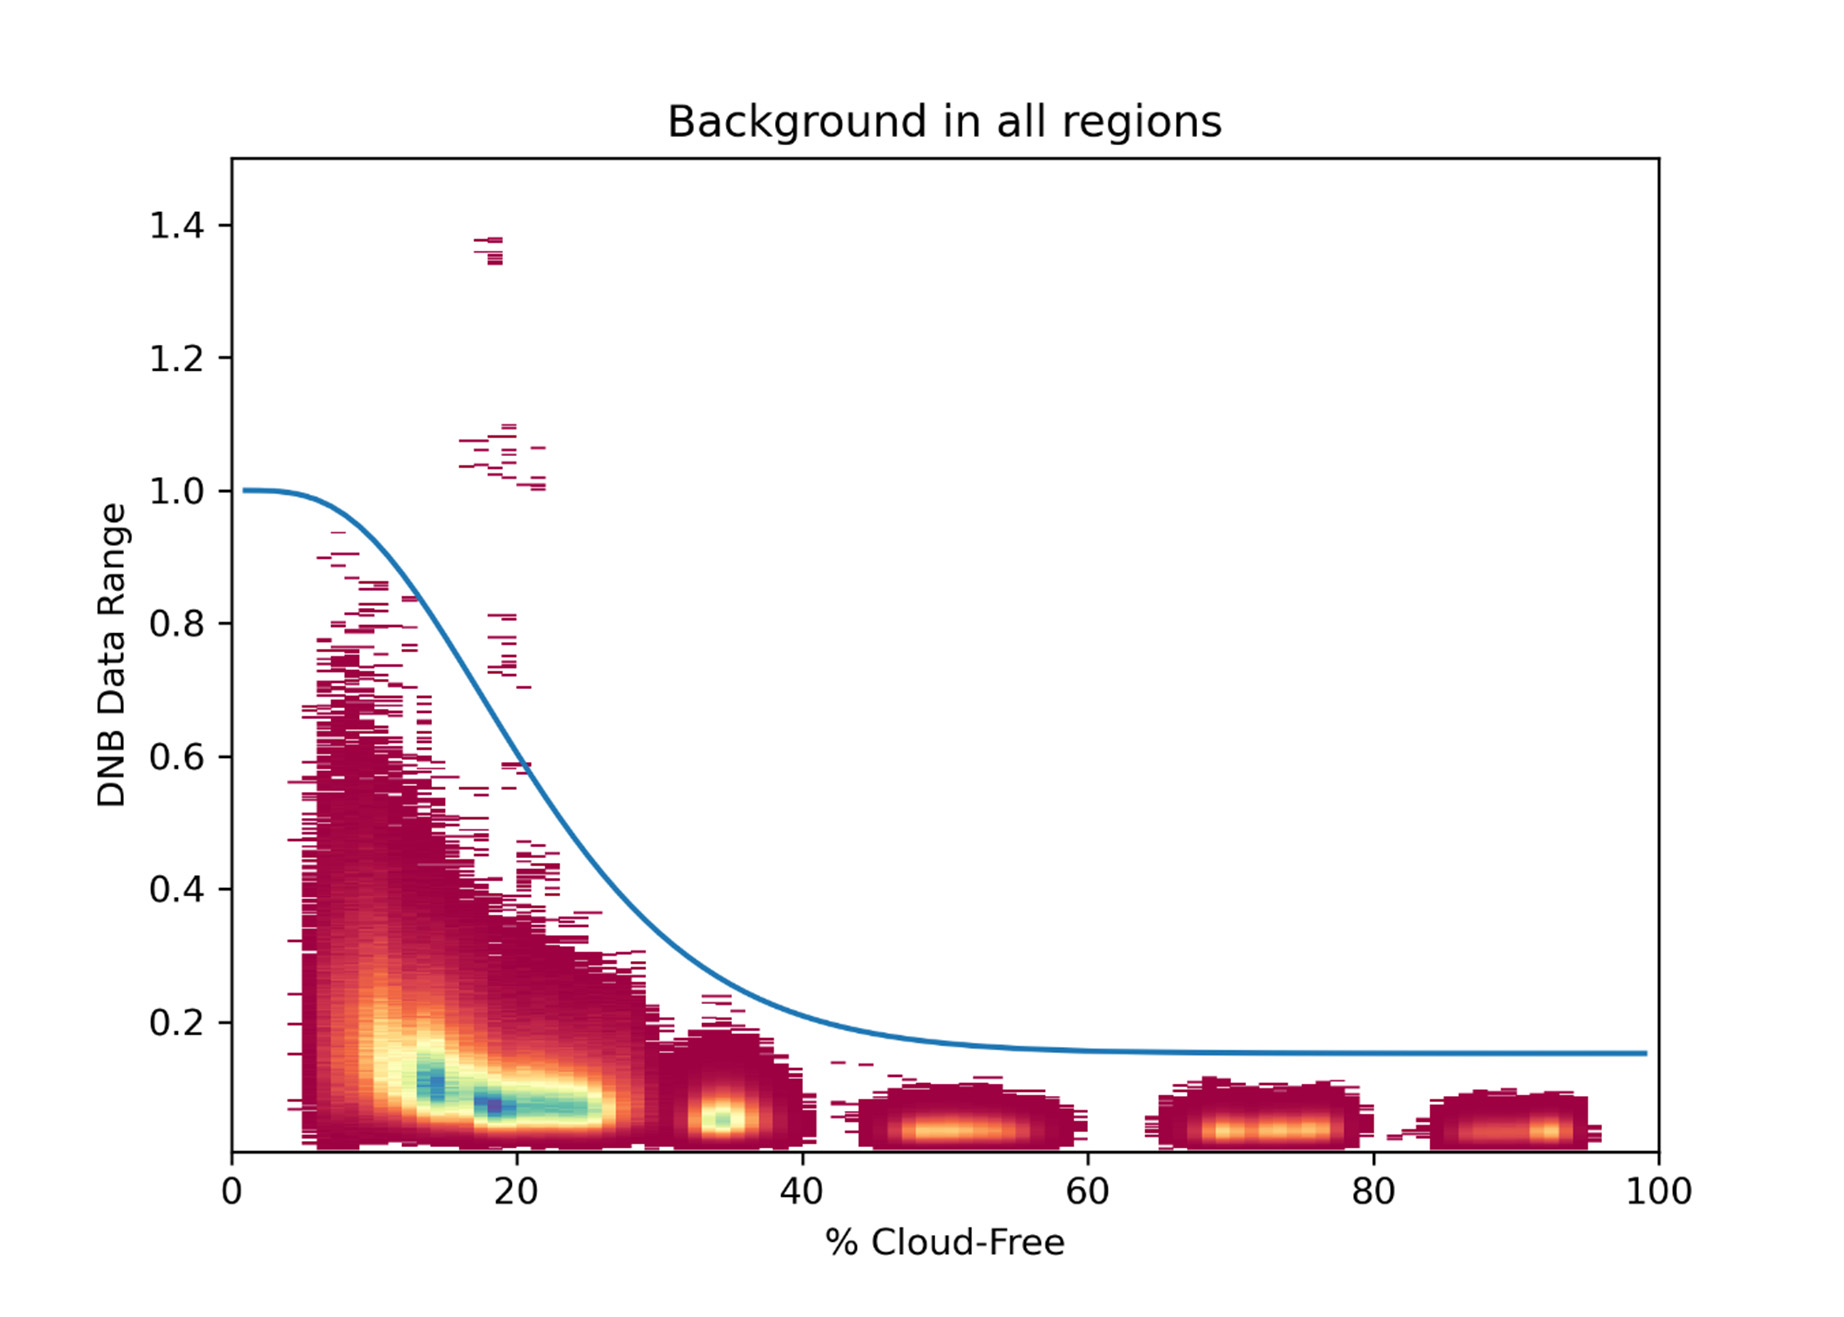
\includegraphics[width=13cm]{images/scattergram.jpg}
    \centering
    \caption{Scattergram and gamma curve - \citep{elvidge2021annual}.}
    \label{fig:scattergram}
\end{figure}

Finally, much noise was caused by the Aurora Borealis. Increasing the threshold too much would have resulted in a significant loss of information in other areas of the globe. Therefore, a \textit{manual} approach was adopted by overlaying a layer on the residual noise in the north and south aurora zones.
As mentioned earlier, although these algorithms \citep{elvidge2021annual} constitute state-of-the-art in the field, they do not correct for some peculiar events. When analysing the data, I found some anomalies. If I extract the maximum observable values, I find very high values in Russia in the middle of nature partly caused by gas flaring, a phenomenon due to the high quantity of natural gas processing plants in the region.
This phenomenon is particularly relevant for the purpose of this thesis because it causes huge light concentrations that leads to pixels 200 times brighter than the most populated capitals in the world. 
These points are few, but they take high values, and the sum extraction process leads to very different results in some countries. In the following sections, I will try to deal with this problem.
Finally, after analysing the data, I found that between 2016 and 2017 there is a big jump in the levels of night-time lights for many countries in the world. The reason seems to be that as of 12 January 2017, the EOG team changed the methodology for converting the raw data to radiance data.
Specifically, the dark offset term used in converting the raw counts to radiance was changed from a dark ocean view to a space view, resulting in a slight upward radiance shift per each data point. This was first documented by \citet{elvidge2020indicators} in which this change was quantified as an increase in the radiance of about $0.125nw/cm^2/sr$. This upward shift led to an overall radiance increase of up to 20\% in some countries.
Since the shift of radiance occurred in the conversion from raw data to radiance data and since I only had access to the latter, I was unable to harmonise the pre-2017 data with the post-2017 data. However, because in this thesis I work with growth rates and not levels, this did not pose any particular problem and dropping the 2017 growth rates observations was sufficient. 
\section{Outliers} 
A quick analysis of the data shows that the brightness of a city of 500,000 to 1 million inhabitants reaches maximum values of between $100$ and $250nW/cm^2/sr$. The city of Milan, one of the brightest places in Italy, reaches maximum values of $130/140nW/cm^2/sr$ in the centre and around $200nW/cm^2/sr$ at its airports. Other European cities have similar characteristics, with London reaching maximums of $200/240nW/cm^2/sr$ in the area around Piccadilly and Oxford Circus, and Paris and Rome reaching values of no more than $120/150nW/cm^2/sr$ in the centre. American cities, which are generally considered brighter, reach higher values. The brightest point in New York is the block between the Rockefeller centre and Time Square, which reaches a peak of about $420nW/cm^2/sr$. These values are similar with the largest world capitals, which are generally considered bright. Dubai is generally less bright than New York except for the pixel containing the Burj Kalifa, the world's tallest skyscraper, which reaches brightness levels of over $500nW/cm^2/sr$. Asian cities are all comparable with New York but, in the vast majority of cases, emit lower light peaks. Hong Kong, for example, does not exceed $220nW/cm^2/sr$, Shenzen $100nW/cm^2/sr$, very similar to Milan, while Tokyo, the brightest of the Asian cities, barely exceeds $400nW/cm^2/sr$.

The brightest city in the world is undoubtedly Las Vegas, the average value in the city centre is around $1,000nW/cm^2/sr$ in an area of about 11 square kilometres. In addition, the pixel containing The Luxor Hotel & Casino reaches a peak of $6,000nW/cm^2/sr$. The reason is quickly stated, the pyramid-shaped hotel emits a beam of light at its apex that is directed towards the sky. I conjecture that these values may be considered too extreme to have an economic relevance on GDP and that perhaps they should be handled as outliers. But they are not alone.

 Russia is one of the countries whose images suffer most from extreme values. Looking at night-time images of Russia, multiple pixels with values totally out of scale can be observed. Namely, pixels with values of more than $10,000nW/cm^2/sr$ in the middle of nowhere, tens of kilometres away from population centres.
Studying point by point, I found two interesting phenomena. The first confirmed, as mentioned before, that Russia is indeed dotted with gas flares, which are fields with vents burning day and night. The second is that, surprisingly, these flames are exceeded in light output by building similar to sheds in the middle of the steppe. I cross-referenced OpenStreetMap data and some Google searches, discovering that such sheds are indeed greenhouses  with controlled environment agriculture. They consist in transparent structures with artificial illumination to boost plants growth.
Russia's solid agricultural vocation, with limited energy costs, has led to the flourishing of many greenhouses heated and illuminated by thousands, but perhaps millions, of light bulbs turned on day and night. 
\begin{figure}
    \hspace*{-1.8cm}
    \centering
    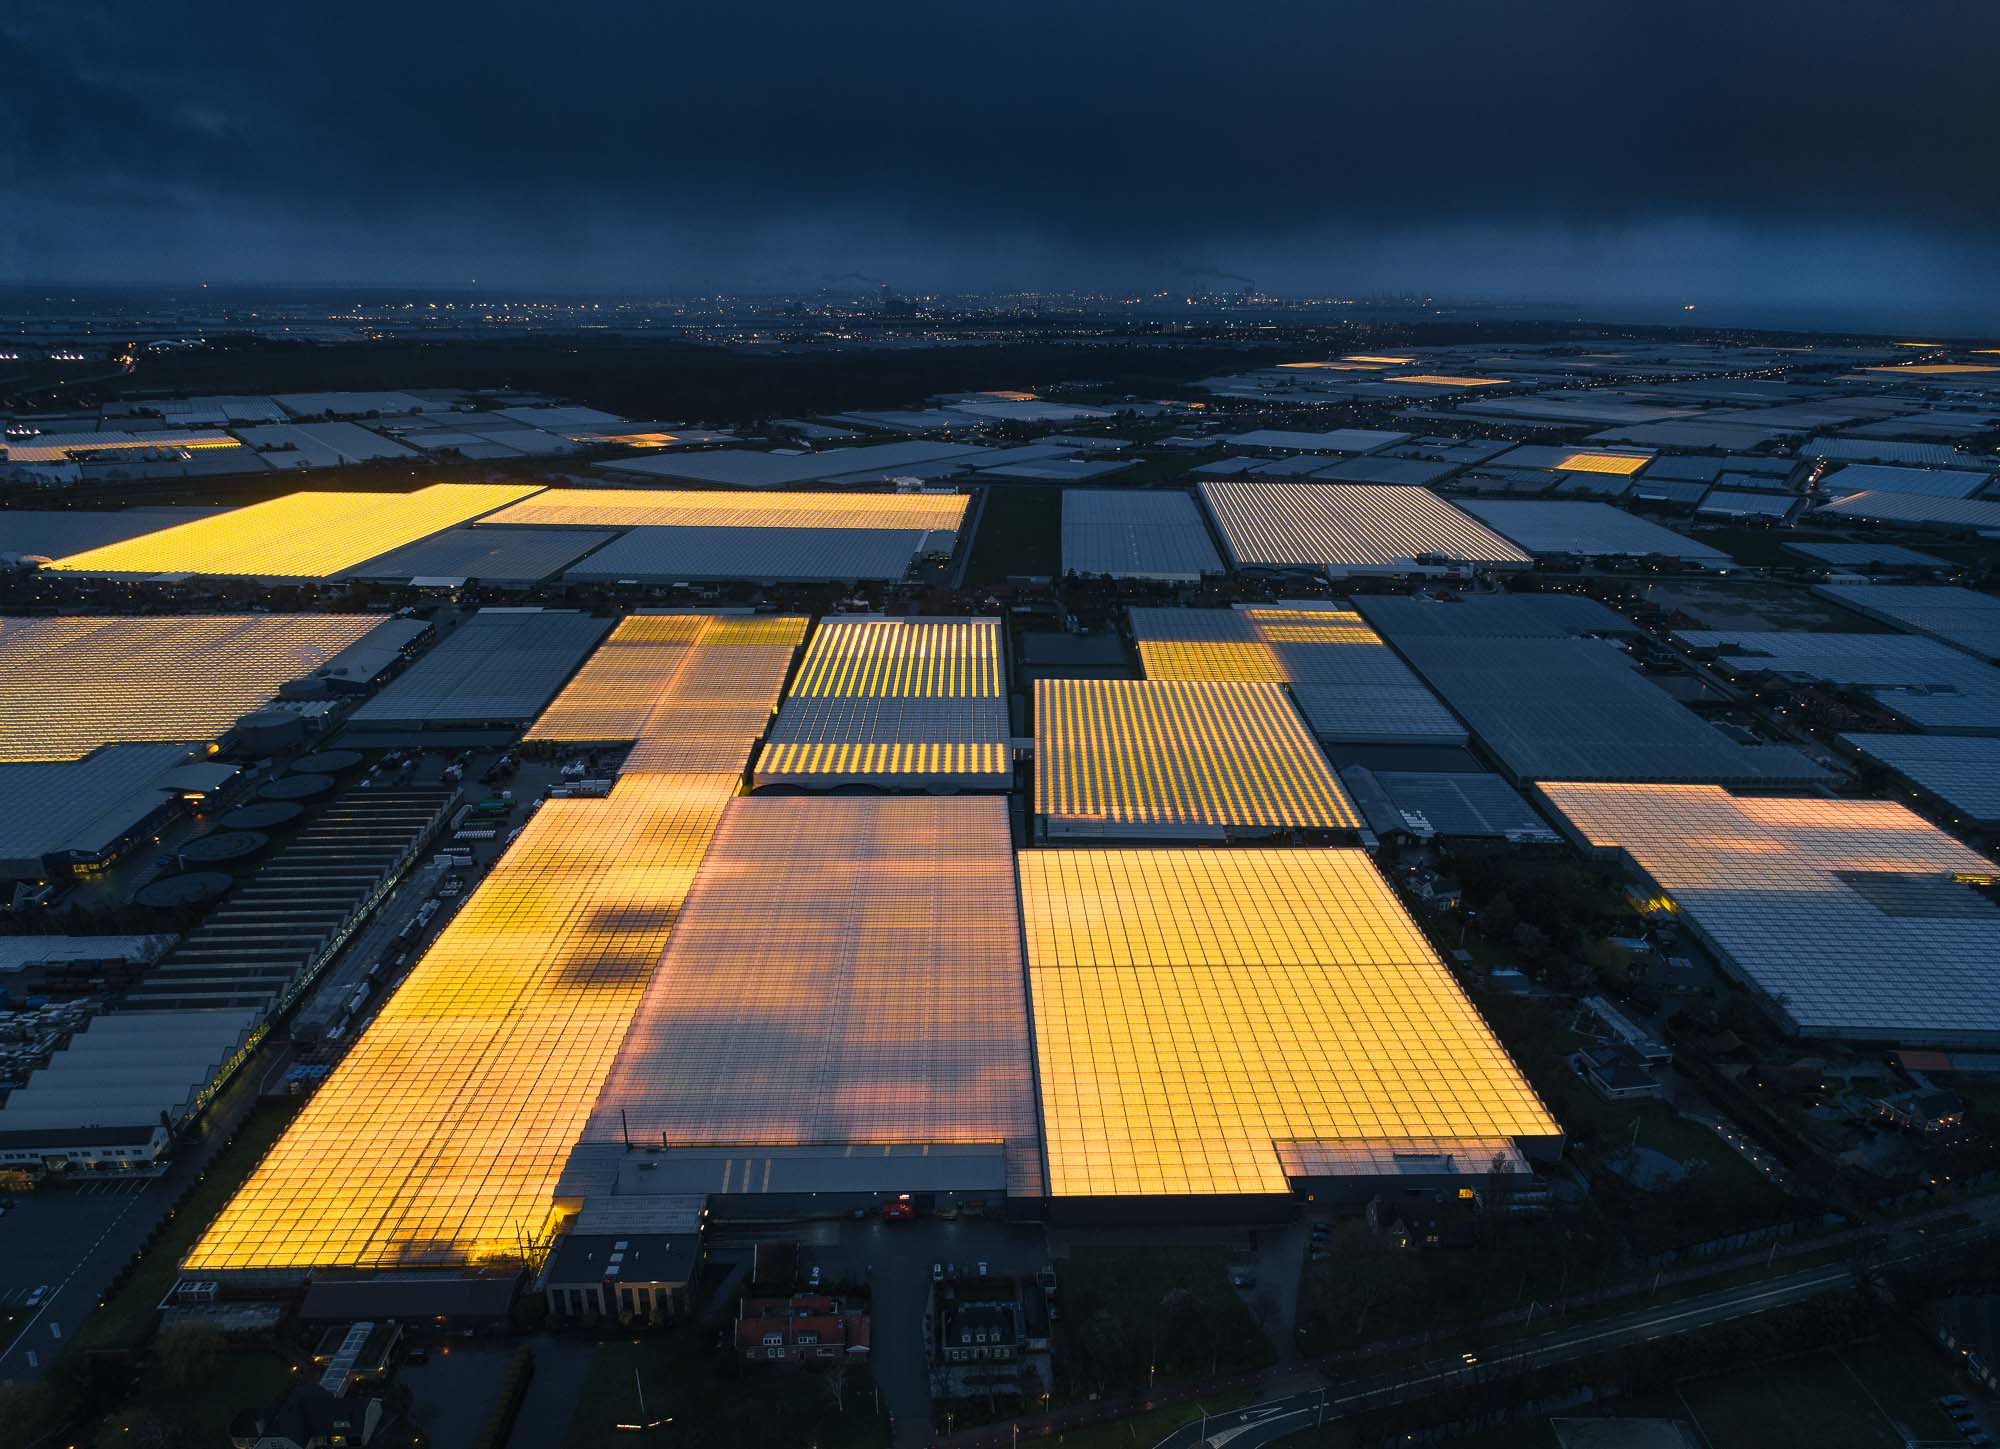
\includegraphics[width=15cm]{images/greenhousehegen.jpg}
    \caption{Netherlands' greenhouses with controlled environment agriculture - Tom Hegen (2019).}
    \label{fig:my_label}
\end{figure}
The transparent roofs with the huge amount of light make these greenhouses some of the brightest places on Earth. This kind of greenhouse can also be found outside Russia because all countries with high latitudes need to compensate for the lack of daylight, especially during the winter. To my knowledge, greenhouses never appear in the literature, even though it is a significant problem that needs to be addressed when dealing with night-time lights for economic applications. In 2021, the total light emitted by Russia cleaned by these two phenomena was about 20\% less than the un-cleaned imagery. A vast difference that, however, seems to be extremely invasive for Russia only. In other European countries, this phenomenon is much more limited. In Italy, for example, such outliers cannot be observed, not even in Spain, France and Germany. The only exception is the Netherlands, which has several greenhouses of the same Russian technology, albeit in smaller quantities.
Concerning gas flares, on the other hand, I found no outliers in Europe with the same Russian magnitude. On the contrary north African countries, endowed with well-known oil deposits, are full of them. 

Dealing with these outliers raises some critical economic questions. Greenhouses and gas flares enter directly into the GDP count. It is, therefore, questionable whether it is correct to eliminate or keep them. However, it is unrealistic to think that a pipeline vent in Siberia that emits as much light as an average European metropolis has the same impact on GDP. Therefore, I decided to clean the data from outliers but keep the original data, which will be compared on the following pages. 

\subsection{Outlier Removal strategies}

Several strategies are adopted to deal with outliers:
\begin{enumerate}
    \item Spatial correction: the algorithm checks each pixel and compares it with the surrounding area, usually $3\times3$ or $5\times5$ pixels. If the value of the pixel is several orders of magnitude higher than the average of the surrounding area, the pixel is recognised as an outlier and is removed
    \item Statistical correction: a predetermined percentile of the data distribution is removed. (For data from Russia, tests suggest the removal of the 0.001 tail)
    \item Manual correction: By looking at the values of cities and the central infrastructure of a country (airports, first of all), it is possible to derive a maximum threshold beyond which all other data are outliers. As far as Russia is concerned, the maximum value observed in cities is less than 500, while all values above are greenhouses or gas flares.
\end{enumerate}

For reasons of computational power, in this thesis, I will use the third approach since it appears to be sufficient. Moreover, power and RAM at a server level are required to manipulate this type of data.
%*****************************************
%*****************************************
%*****************************************
%*****************************************
%*****************************************